% Source: AESP_466_ClassWork/Supplements/Companion/Euler_Sequences_Quaternions/Euler_Sequences_Quaternions.tex

\documentclass[border=4pt]{standalone}
\usepackage{amsmath}
\usepackage{amssymb}
\usepackage{graphicx}
\usepackage{tikz}
\usepackage{xcolor}
\usetikzlibrary{shapes.geometric, arrows.meta, positioning, decorations.pathmorphing, decorations.pathreplacing, patterns, calc, 3d}

\definecolor{Garnet}{HTML}{73000A}
\definecolor{USC_Rose}{HTML}{CC2E40}
\definecolor{USC_Blue}{HTML}{466A9F}
\definecolor{USC_Slate}{HTML}{1F414D}
\definecolor{USC_Olive}{HTML}{65780B}
\definecolor{USC_Lime}{HTML}{CED318}
\definecolor{USC_Gold}{HTML}{A49137}
\definecolor{USC_Black90}{HTML}{565656}
\definecolor{USC_Black10}{HTML}{ECECEC}

\newcommand{\sectionheader}[1]{%
  \vspace{0.5cm}
  {\noindent\Large \textbf{#1}}
  \vspace{0.2cm}
  \hrule
  \vspace{0.1cm}
  \hrule
  \vspace{0.3cm}
}

\begin{document}
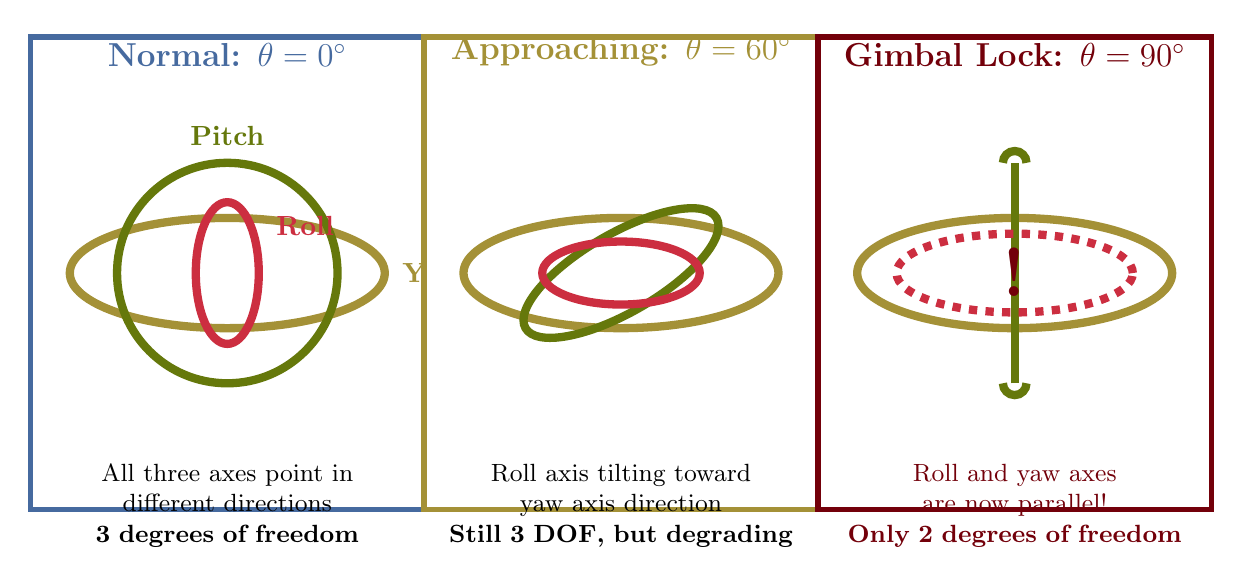
\begin{tikzpicture}[scale=1.0]
    % Normal case
    \begin{scope}[shift={(-5,0)}]
        \draw[draw=USC_Blue, line width=2pt, fill=white] (-2.5,-3) rectangle (2.5,3);
        \node[above, font=\bfseries\large, USC_Blue] at (0,2.5) {Normal: $\theta = 0^\circ$};

        % Draw gimbal rings
        % Outer ring (yaw - z)
        \draw[line width=3pt, USC_Gold] (0,0) ellipse (2 and 0.7);
        \node[USC_Gold, font=\bfseries, right] at (2.1,0) {Yaw};

        % Middle ring (pitch - y) - tilted
        \draw[line width=3pt, USC_Olive] (0,0) ellipse (1.4 and 1.4);
        \node[USC_Olive, font=\bfseries, above] at (0,1.5) {Pitch};

        % Inner ring (roll - x) - more tilted
        \draw[line width=3pt, USC_Rose] (0,0) ellipse (0.4 and 0.9);
        \node[USC_Rose, font=\bfseries, right] at (0.5,0.6) {Roll};

        \node[below, text width=4.5cm, align=center, font=\small] at (0,-2.3) {All three axes point in\\different directions\\{\bfseries 3 degrees of freedom}};
    \end{scope}

    % Intermediate case
    \begin{scope}[shift={(0,0)}]
        \draw[draw=USC_Gold, line width=2pt, fill=white] (-2.5,-3) rectangle (2.5,3);
        \node[above, font=\bfseries\large, USC_Gold] at (0,2.5) {Approaching: $\theta = 60^\circ$};

        % Outer ring (yaw - z) - still horizontal
        \draw[line width=3pt, USC_Gold] (0,0) ellipse (2 and 0.7);

        % Middle ring (pitch - y) - tilted forward
        \begin{scope}[rotate=30]
            \draw[line width=3pt, USC_Olive] (0,0) ellipse (1.4 and 0.5);
        \end{scope}

        % Inner ring (roll - x) - starting to align with yaw
        \draw[line width=3pt, USC_Rose] (0,0) ellipse (1.0 and 0.4);

        \node[below, text width=4.5cm, align=center, font=\small] at (0,-2.3) {Roll axis tilting toward\\yaw axis direction\\{\bfseries Still 3 DOF, but degrading}};
    \end{scope}

    % Gimbal lock case
    \begin{scope}[shift={(5,0)}]
        \draw[draw=Garnet, line width=2pt, fill=white] (-2.5,-3) rectangle (2.5,3);
        \node[above, font=\bfseries\large, Garnet] at (0,2.5) {Gimbal Lock: $\theta = 90^\circ$};

        % Outer ring (yaw - z) - horizontal
        \draw[line width=3pt, USC_Gold] (0,0) ellipse (2 and 0.7);

        % Middle ring (pitch - y) - now vertical
        \draw[line width=3pt, USC_Olive] (0,-1.4) -- (0,1.4);
        \draw[line width=3pt, USC_Olive] (-0.15,-1.4) arc (180:360:0.15);
        \draw[line width=3pt, USC_Olive] (-0.15,1.4) arc (180:0:0.15);

        % Inner ring (roll - x) - NOW ALIGNED WITH YAW!
        \draw[line width=3pt, USC_Rose, dashed] (0,0) ellipse (1.5 and 0.5);

        % Big warning
        \node[Garnet, font=\Huge\bfseries] at (0,0) {!};

        \node[below, text width=4.5cm, align=center, font=\small, Garnet] at (0,-2.3) {Roll and yaw axes\\are now parallel!\\{\bfseries Only 2 degrees of freedom}};
    \end{scope}
\end{tikzpicture}
\end{document}
